\section{Metodologia}

Foram utilizadas as câmeras principal, no modo 1x (\texttt{cam1}), e ultrawide,
no modo 0,5x (\texttt{cam05}), de um Samsung Galaxy A56. A coleta inicial reuniu
22 fotografias do tabuleiro por câmera, com resolução de $2992\times2992$ pixels,
variando posição, distância e inclinação do padrão. O tabuleiro possui
$5\times5$ quadrados de lado $3{,}1$~cm e $4\times4$ cantos internos. Os dados
foram organizados em diretórios independentes para cada câmera.
Para avaliar a projeção, foram obtidas outras três fotografias do tabuleiro por
câmera, armazenadas em \texttt{project\_test/} e mantidas fora da calibração.

A implementação utiliza Python, NumPy e OpenCV. Em \texttt{calibrate.py}, os
cantos são detectados com \texttt{cv2.findChessboardCorners()}, com
\texttt{cv2.findChessboardCornersSB()} como alternativa em caso de falha, e
refinados por \texttt{cv2.cornerSubPix()}. O refinamento utiliza janela de
$11\times11$ pixels, limite de 30 iterações e tolerância de $0{,}001$ pixel.
A Figura~\ref{fig:corners} apresenta uma detecção existente no repositório.

A calibração utiliza \texttt{cv2.calibrateCamera()}, que recebe as coordenadas
do padrão e as observações 2D. Em seguida, \texttt{undistort.py} aplica
\texttt{cv2.undistort()} às fotografias, enquanto \texttt{project.py} estima
a pose com \texttt{cv2.solvePnP()} e calcula projeções com
\texttt{cv2.projectPoints()}. Todos os cálculos utilizam a resolução original;
os detalhes ampliados nas figuras servem apenas à apresentação.

\begin{figure}[H]
  \centering
  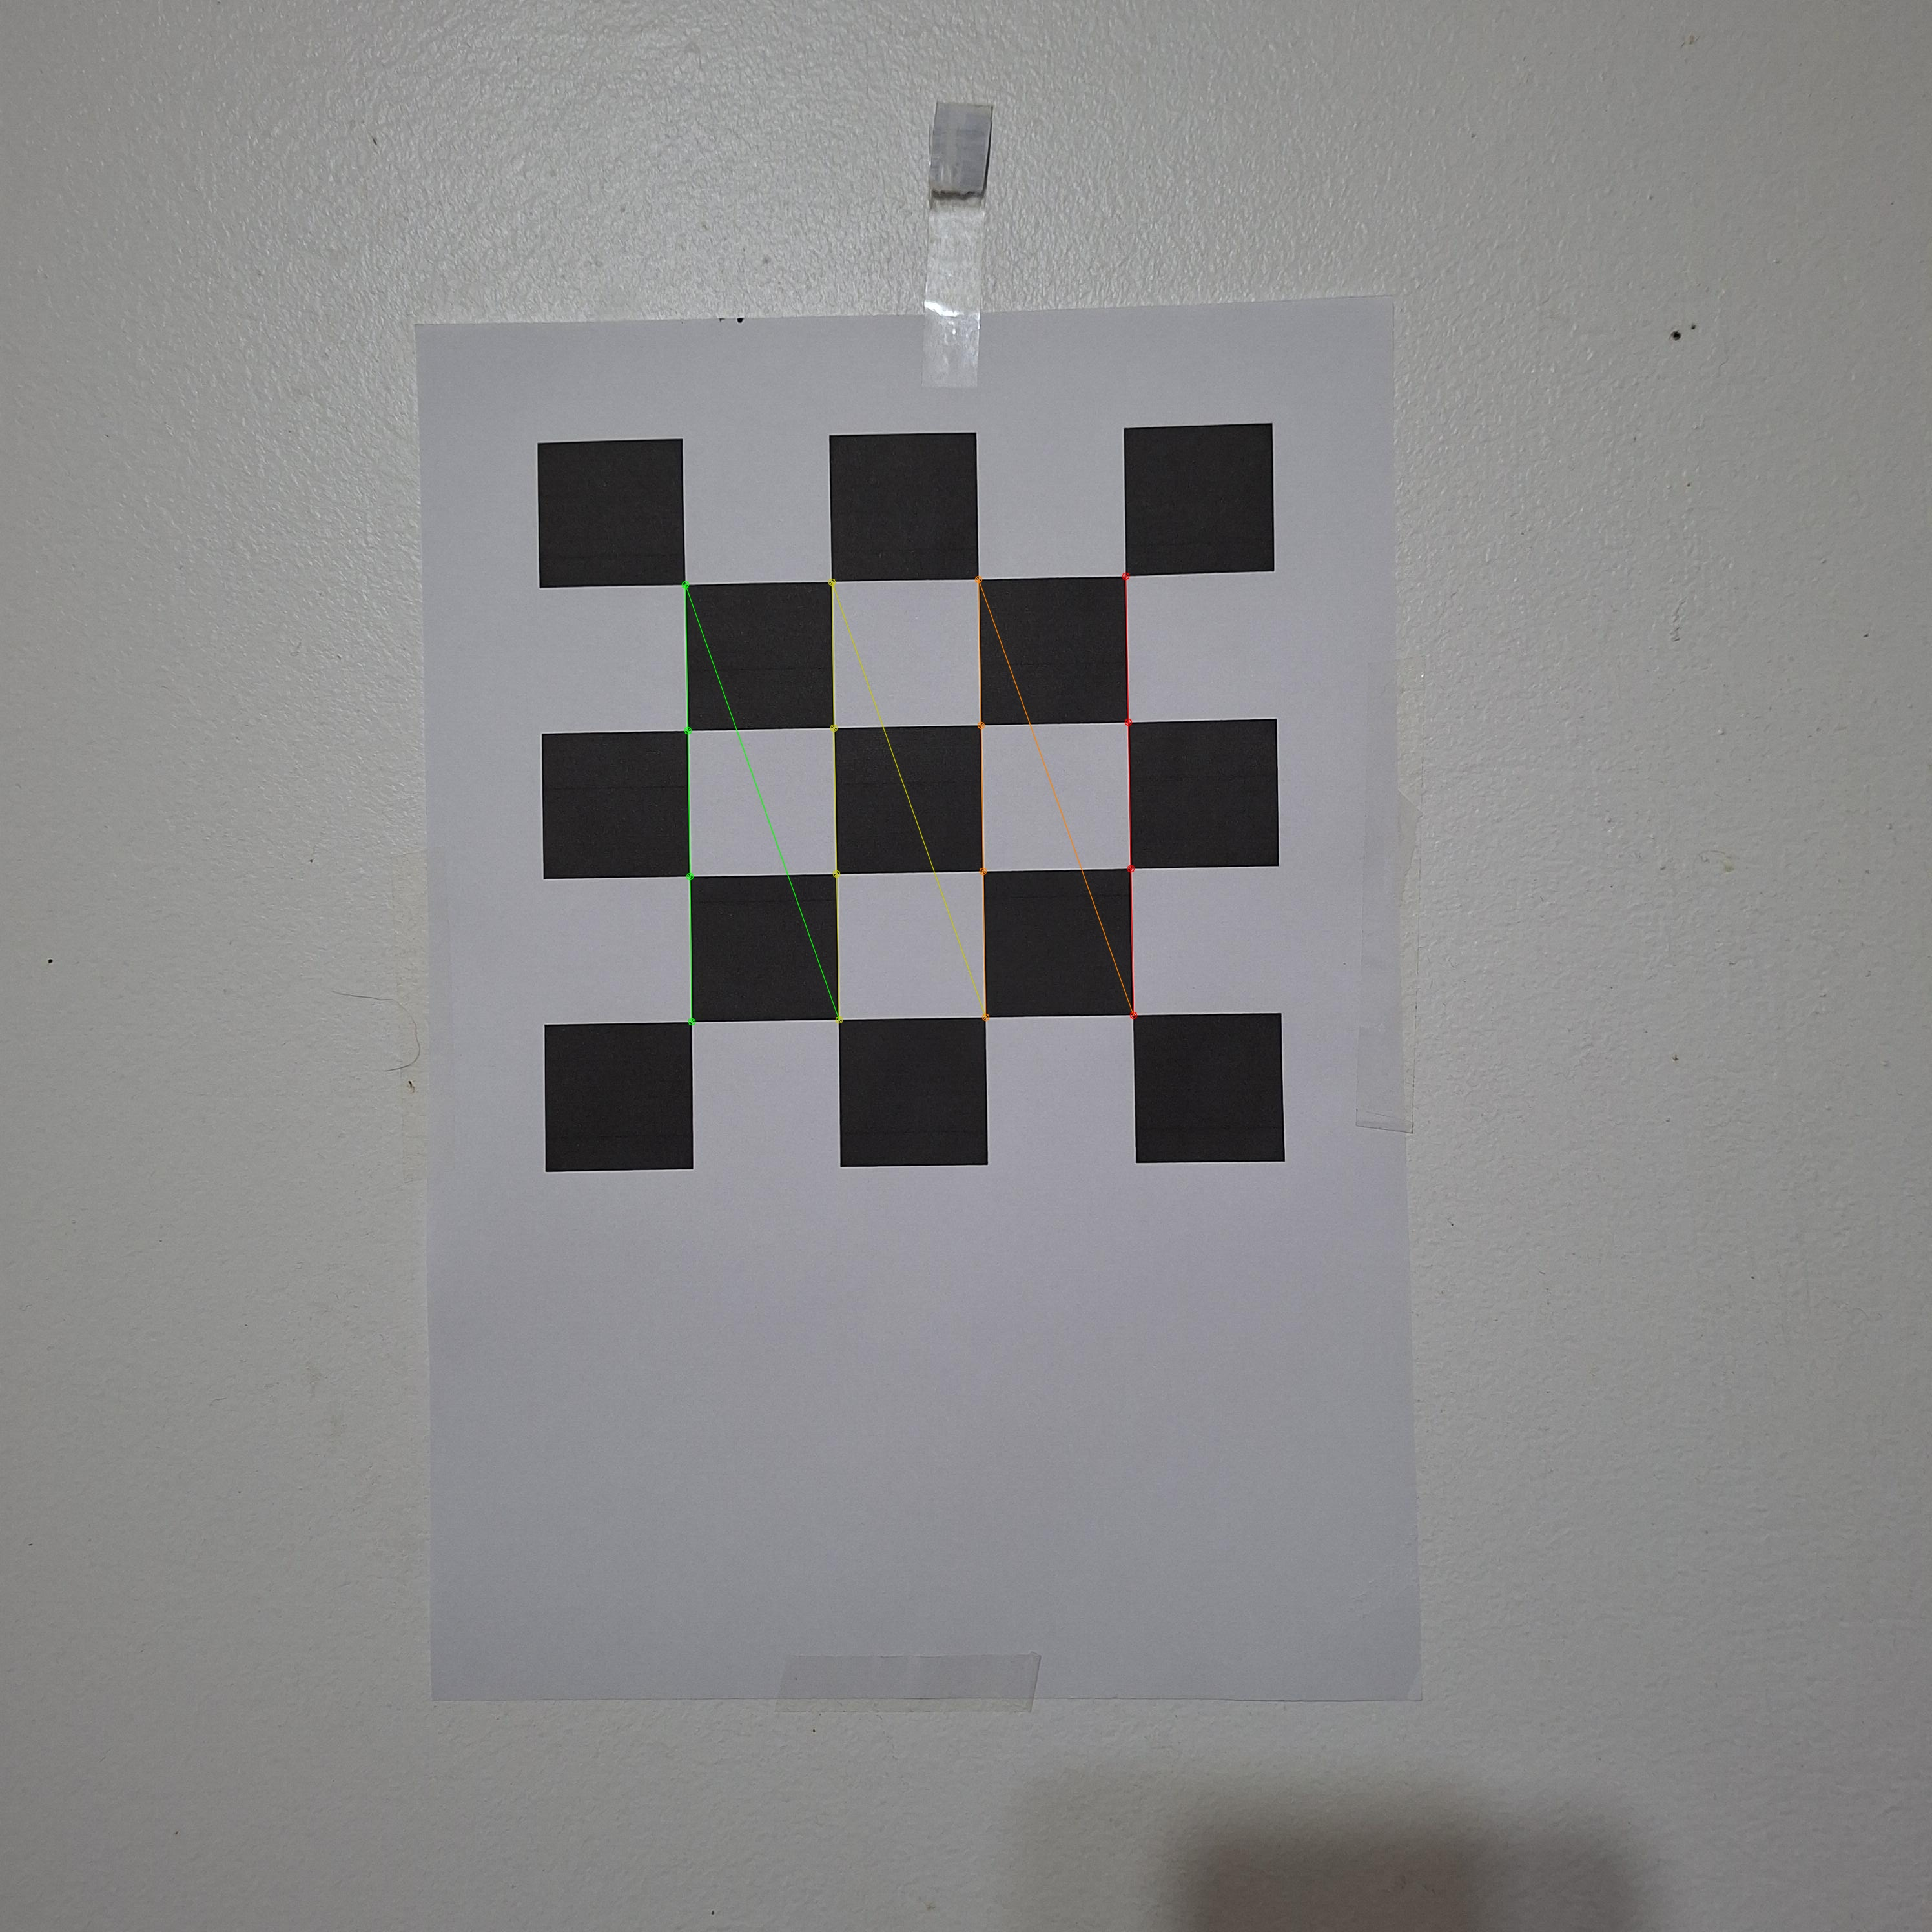
\includegraphics[width=0.39\linewidth,trim=650bp 942bp 792bp 480bp,clip]{board-corners.jpg}
  \caption{Detalhe da fotografia \texttt{001.jpg} da câmera 1x, com os 16 cantos
  internos detectados e conectados pelo OpenCV.}
  \label{fig:corners}
\end{figure}
